%%%%%%%%%%%%%%%%%%%%%%%%%%%%%%%%%%%
%%%  Filename: thesis_template.tex
%%%  ---
%%%  Template for Master Thesis at DTETI UGM   		
%%%  Created using thesisdtetiugm.cls
%%%  --- 
%%%  Written by Canggih Puspo Wibowo
%%%  [canggihpw@gmail.com]
%%%%%%%%%%%%%%%%%%%%%%%%%%%%%%%%%%%

%% Use option "bahasa" or "english" 
%%    to change the basic language used
%% User option "bachelor", "master", or "doctoral"
%% 	  to change the degree
% \documentclass[<bachelor/master/doctoral>,<bahasa/english>]{thesisdtetiugm}
\documentclass[bachelor,bahasa]{thesisdtetiugm}
%\documentclass[bachelor,english]{thesisdtetiugm}
%======================================
% Information Input
%======================================
% Input author's name and ID number
\author{AHMAD ZAKI AKMAL}{21/480179/TK/52981}
% Input the thesis' title
\title{FAULT-TOLERANT WEB SERVICES USING BLOCKCHAIN}
% Program and the head of the program
\program{TEKNOLOGI INFORMASI}{<<Program coordinator>>}{<<NIP>>}
% Name of department head and NIP
\departmenthead{<<Head of the department>>}{<<NIP>>}
\major{INFORMATION ENGINEERING}
\yearsubmit{<<TAHUN PENDADARAN>>}
\examdate{<<Exam date>>}
% Name of thesis supervisors/promotors
\addsupervisor{Guntur Dharma Putra, PhD.}{<<NIP xxxxxx>>}
\addsupervisor{Azkario Rizky Pratama, ST, M.Eng., Ph.D.}{<<NIP xxxxxx>>}
%\addsupervisor{<<Supervisor 3>>}{<<NIP>>}
% Name of examiners
%\addexaminer{<<Examiner 1>>}{<<NIP 1>>}
%\addexaminer{<<Examiner 2>>}{<<NIP 2>>}
%\addexaminer{<<Examiner 3>>}{<<NIP 3>>}
%\addexaminer{<<Examiner 4>>}{<<NIP 4>>}
%\addexaminer{<<Examiner 5>>}{<<NIP 5>>}
%\addexaminer{<<Examiner 6>>}{<<NIP 6>>}
%\addexaminer{<<Examiner 7>>}{<<NIP 7>>}
%\addexaminer{<<Examiner 8>>}{<<NIP 8>>}
%\addexaminer{<<Examiner 9>>}{<<NIP 9>>}

%======================================

% correct bad hyphenation here [example]
% \babelhyphenation[<<english/bahasa>>]{op-tical net-works semi-conduc-tor}
%% Uncomment block of code below to disable hyphenation
%\tolerance=1
%\emergencystretch=\maxdimen
%\hyphenpenalty=10000
%\hbadness=10000

\begin{document}
%======================================
% Create cover etc
%======================================

%---- COVER ----
%\printcover{sample/logougm.png}{Pendadaran/Tesis/Ringkasan Tesis*}
\printcover{sample/logougm.png}{Bachelor}
% *Choose one

%---- ENDORSEMENT PAGE ----
% Select endorsement page type. If you want to use your own PDF file,  
% 	use \printendorsementpdf, or if you want to use JPG file, use 
% 	\printendorsementjpg. Otherwise, use \printendorsement.
% 	Choose one only. Comment out unused command(s).
%
\cleardoublepage \phantomsection
\printendorsement
%\printendorsementpdf
%\printendorsementjpg{sample/scanned-endorsement.jpg}

%---- DEDICATION PAGE ----
\cleardoublepage \phantomsection
\chapterstatement{contents/statement/statement}
%\chapterstatementjpg{sample/scanned-statement.jpg}

\cleardoublepage \phantomsection
\chapterdedication{contents/dedication/dedication}

%---- STATEMENT PAGE ----
% Select statement page type. If you want to use your own JPG file,  
%	use \chapterstatementjpg{<your *.jpg file path>}. Otherwise, 
%	use \chapterstatement{contents/statement/statement}.
%	Choose one only. Comment out unused command(s).
%


%---- PREFACE PAGE ----
\cleardoublepage \phantomsection
\chapterpreface{contents/preface/preface}

%======================================
% Create Table of Contents, List of Figures, List of Tables
% <Do not change this part>
%======================================
\cleardoublepage \phantomsection
\thetoc
\onehalfspacing
\tableofcontents
\singlespacing
\cleardoublepage \phantomsection
\thelot
\listoftables
\cleardoublepage \phantomsection
\thelof
\listoffigures

%======================================

%---- NOMENCLATURE PAGE ----
\cleardoublepage \phantomsection
\chapternomenclature{contents/nomenclature/nomenclature}

%---- INTISARI PAGE----
\cleardoublepage \phantomsection
\chapterintisari{contents/abstract/intisari}

%---- ABSTRACT PAGE----
\cleardoublepage \phantomsection
\chapterabstract{contents/abstract/abstract}


%======================================



%======================================
%  MAIN TEXT
%======================================
\startmain
% You can change 
%    the filename and location of the files inputted
\cleardoublepage \phantomsection
\chapter{Pendahuluan}

\section{Latar Belakang}

Sub-bab ini berisi uraian tentang latar belakang atau justifikasi ilmiah dan permasalahan yang akan diteliti, alasan penelitian dan penelitian yang pernah dilakukan sebelumnya terkait fenomena tersebut.

%HAPUS YANG TIDAK PERLU
%-------------------------------------------------
\noindent\textbf{Contoh latar belakang penelitian untuk teknik elektro:} \\
\noindent\fbox{%
	\parbox{\textwidth}{%
				
		\hspace{1cm} "Peningkatan konsumsi energi listrik yang terus menerus menyebabkan ketersediaan 
		sumber energi yang semakin terbatas. Sumber energi terbarukan seperti solar dan angin 
		menjadi solusi yang menjanjikan untuk memenuhi kebutuhan energi. Namun, kapasitas 
		produksi dan efisiensi dari sumber energi terbarukan masih sangat tergantung pada 
		kondisi cuaca dan geografis. Oleh karena itu, perlu adanya sistem penyimpanan energi 
		yang efisien dan dapat memastikan ketersediaan energi listrik secara kontinu. Penelitian 
		ini akan mengevaluasi kemampuan superkapasitor dalam menyimpan dan mengirimkan 
		energi secara efisien dan memastikan ketersediaan energi listrik secara kontinu."
		
	}%
}

%-------------------------------------------------	
\vspace{5mm}
Latar belakang ini memperkenalkan masalah ketersediaan sumber energi dan 
peningkatan konsumsi energi listrik yang terus menerus. Ini juga memperkenalkan solusi 
yang menjanjikan dari sumber energi terbarukan dan menjelaskan mengapa perlu adanya 
sistem penyimpanan energi yang efisien. Latar belakang ini memberikan dasar yang kuat 
bagi perumusan masalah dan tujuan penelitian, memastikan bahwa hasil penelitian 
memiliki relevansi dan signifikansi bagi bidang terkait.

%HAPUS YANG TIDAK PERLU
%-------------------------------------------------
\noindent\textbf{Contoh latar belakang penelitian untuk teknik biomedis:} \\
\noindent\fbox{%
	\parbox{\textwidth}{%
		
		\hspace{1cm} "Diagnosis dan pengobatan penyakit memerlukan integrasi informasi medis yang 
		akurat dan terkini. Alat diagnostik tradisional seperti CT scan dan MRI memiliki resolusi 
		yang tinggi dan dapat mengidentifikasi masalah pada tingkat sel, tetapi sering 
		memerlukan banyak waktu dan biaya. Alat deteksi dini seperti tes darah dan urin memiliki 
		biaya rendah dan mudah digunakan, tetapi sering kurang akurat dan tidak memberikan gambaran yang jelas tentang masalah medis. Oleh karena itu, penting untuk menemukan metode baru yang memadukan keunggulan dari kedua jenis alat tersebut. Penelitian ini akan mengevaluasi kemampuan nanopartikel dalam meningkatkan akurasi dan efisiensi diagnosis medis."
		
	}%
}

%-------------------------------------------------	
\vspace{5mm}
Latar belakang ini memperkenalkan masalah diagnostik dan pengobatan penyakit dan mempertimbangkan pentingnya integrasi informasi medis yang akurat dan terkini. Ini 
juga memperkenalkan kelemahan dari alat diagnostik tradisional dan deteksi dini dan menjelaskan mengapa penting untuk menemukan metode baru yang memadukan 
keunggulan dari kedua jenis alat tersebut. Latar belakang ini memberikan dasar yang kuat bagi perumusan masalah dan tujuan penelitian, memastikan bahwa hasil penelitian 
memiliki relevansi dan signifikansi bagi bidang terkait.

%HAPUS YANG TIDAK PERLU
%-------------------------------------------------
\noindent\textbf{Contoh latar belakang penelitian untuk teknologi informasi:} \\
\noindent\fbox{%
	\parbox{\textwidth}{%
		
\hspace{1cm} "Dengan perkembangan teknologi informasi yang sangat pesat dalam beberapa tahun terakhir, penyimpanan data menjadi masalah yang semakin penting. Semakin banyak data yang diterima setiap hari, semakin penting bagi organisasi untuk memastikan bahwa data 
mereka aman dan terlindungi. Pada saat yang sama, organisasi juga membutuhkan akses cepat dan efisien ke data mereka untuk membuat keputusan yang tepat. Teknologi 
enkripsi kuantum baru-baru ini muncul sebagai solusi potensial untuk memenuhi kebutuhan ini, dengan menawarkan tingkat keamanan yang jauh lebih tinggi dan proses 
enkripsi yang lebih cepat dibandingkan dengan teknologi enkripsi konvensional. Oleh karena itu, penting untuk mengevaluasi efektivitas dan keamanan teknologi enkripsi 
kuantum dalam sistem penyimpanan data cloud."
		
	}%
}

%-------------------------------------------------	
\vspace{5mm}
Latar belakang ini memperkenalkan masalah penyimpanan data dan mempertimbangkan pentingnya keamanan data. Ini juga memperkenalkan teknologi enkripsi kuantum sebagai solusi potensial dan menjelaskan mengapa evaluasi teknologi ini penting bagi bidang teknologi informasi. Latar belakang ini memberikan dasar yang kuat bagi perumusan masalah dan tujuan penelitian, memastikan bahwa hasil penelitian memiliki relevansi dan signifikansi bagi bidang terkait.

\section{Rumusan Masalah}

Sub-bab ini berisi poin-poin yang menjelaskan masalah atau isu yang akan diteliti dalam suatu penelitian. Ini mencakup formulasi masalah yang jelas dan spesifik dan 
mempertimbangkan latar belakang dan deskripsi masalah yang terkait yang tertulis Dalam latar belakang pada sub-bab sebelumnya. Perumusan masalah yang baik akan membantu menentukan fokus penelitian dan memberikan dasar untuk tujuan dan hipotesis penelitian. Dalam penelitian, perumusan masalah memainkan peran penting dalam memastikan bahwa hasil penelitian berguna dan relevan untuk masalah yang diteliti.

%-------------------------------------------------
\noindent\fbox{%
	\parbox{\textwidth}{%
\noindent\textbf{Contoh} perumusan masalah untuk \textbf{Teknik Elektro}: \\		

\hspace{1cm} \textbf{"Bagaimana memperbaiki efisiensi penghematan energi pada sistem pencahayaan rumah tangga melalui implementasi teknologi kontrol otomatis?"} \\
	
\hspace{1cm} Perumusan masalah ini jelas dan spesifik dan menentukan fokus penelitian pada perbaikan efisiensi penghematan energi dalam sistem pencahayaan rumah tangga dengan menggunakan teknologi kontrol otomatis. Ini juga mempertimbangkan latar belakang tentang pentingnya penghematan energi dan memberikan solusi praktis melalui implementasi teknologi. Perumusan masalah ini memberikan dasar yang kuat untuk tujuan dan hipotesis penelitian dan memastikan bahwa hasil penelitian akan berguna bagi bidang teknik elektro.
		
	}%
}

%-------------------------------------------------
\noindent\fbox{%
	\parbox{\textwidth}{%
\noindent\textbf{Contoh} perumusan masalah untuk \textbf{Teknik Biomedis}: \\		

\hspace{1cm} \textbf{"Bagaimana memperbaiki akurasi deteksi kanker payudara dengan menggunakan teknologi pemindaian ultrasonografi berbasis AI?"} \\

\hspace{1cm} Perumusan masalah ini jelas dan spesifik dan menentukan fokus penelitian pada 
perbaikan akurasi deteksi kanker payudara dengan menggunakan teknologi pemindaian ultrasonografi berbasis AI. Ini mempertimbangkan latar belakang tentang pentingnya deteksi dini kanker payudara dan memberikan solusi praktis melalui implementasi teknologi. Perumusan masalah ini memberikan dasar yang kuat untuk tujuan dan hipotesis penelitian dan memastikan bahwa hasil penelitian akan berguna bagi bidang teknik biomedis.
		
	}%
}

%-------------------------------------------------	
\noindent\fbox{%
	\parbox{\textwidth}{%
\noindent\textbf{Contoh} perumusan masalah untuk \textbf{Teknologi Informasi}: \\		

\hspace{1cm} \textbf{"Bagaimana meningkatkan efisiensi dan keamanan sistem penyimpanan data cloud melalui implementasi teknologi enkripsi kuantum?"} \\

\hspace{1cm} Perumusan masalah ini jelas dan spesifik dan menentukan fokus penelitian pada peningkatan efisiensi dan keamanan sistem penyimpanan data cloud dengan menggunakan teknologi enkripsi kuantum. Ini mempertimbangkan latar belakang tentang pentingnya keamanan data dan memberikan solusi praktis melalui implementasi teknologi. Perumusan masalah ini memberikan dasar yang kuat untuk tujuan dan hipotesis penelitian dan memastikan bahwa hasil penelitian akan berguna bagi bidang teknologi informasi.
		
	}%
}

%-------------------------------------------------	

\section{Tujuan Penelitian}

Tujuan penelitian pada skripsi Teknik (TE, TB, TIF) adalah menentukan sasaran atau target yang ingin dicapai melalui proses penelitian. Tujuan penelitian bisa beragam sesuai dengan bidang ilmu yang dipelajari, topik penelitian, dan permasalahan yang akan dicari solusinya.

Secara umum, tujuan penelitian pada skripsi bidang teknik adalah untuk:

\begin{itemize}
	\item Mengidentifikasi dan menganalisis masalah atau permasalahan dalam bidang \textit{engineering}.
	\item Meningkatkan pemahaman dan wawasan tentang bidang \textit{engineering} melalui penerapan teori dan metodologi yang sesuai.
	\item Mengembangkan solusi atau produk baru yang inovatif dan efektif dalam 
	bidang \textit{engineering}.
	\item Menunjukkan penerapan prinsip-prinsip keteknikan dalam solusi atau produk yang dikembangkan.
	\item Menjelaskan implikasi dan rekomendasi dari hasil penelitian bagi bidang \textit{engineering} dan masyarakat.
\end{itemize}

\begin{minipage}{0.92\textwidth}
Catatan: Tujuan penelitian dalam skripsi bidang teknik harus jelas, spesifik, terukur, dan dapat dicapai dalam jangka waktu yang ditentukan.
\end{minipage}

\newpage
\vspace{5mm}
\textbf{Contoh Tujuan Penelitian Skripsi Teknik Elektro:}

\begin{minipage}{0.92\textwidth}
Berikut adalah beberapa contoh tujuan penelitian yang sesuai dengan topik 
“perbaikan efisiensi penghematan energi pada sistem pencahayaan rumah tangga 
melalui implementasi teknologi kontrol otomatis”:
\end{minipage}

%-------------------------------------------------	
\noindent\fbox{%
	\parbox{\textwidth}{%
\begin{enumerate}
\item Menganalisis tingkat efisiensi energi pada sistem pencahayaan rumah tangga 
sebelum dan setelah implementasi teknologi kontrol otomatis.
\item Mengukur pengurangan biaya listrik setelah implementasi teknologi kontrol 
otomatis pada sistem pencahayaan rumah tangga.
\item Menunjukkan bagaimana teknologi kontrol otomatis dapat memperbaiki 
efisiensi penghematan energi pada sistem pencahayaan rumah tangga.
\item Meningkatkan kenyamanan dan keamanan pengguna rumah tangga melalui 
penggunaan teknologi kontrol otomatis pada sistem pencahayaan.
\item Menjelaskan bagaimana implementasi teknologi kontrol otomatis 
mempengaruhi kualitas cahaya dan faktor-faktor lain dalam sistem pencahayaan 
rumah tangga.
\item Membandingkan efisiensi energi dan biaya pada sistem pencahayaan rumah 
tangga dengan teknologi kontrol otomatis dan sistem manual.
\item Menunjukkan implikasi dan rekomendasi dari hasil penelitian bagi rumah tangga 
dan lingkungan.
\end{enumerate}
		
	}%
}

%-------------------------------------------------	

\newpage
\vspace{5mm}
\textbf{Contoh Tujuan Penelitian Skripsi Teknik Biomedis:}

\begin{minipage}{0.92\textwidth}
Berikut adalah beberapa contoh tujuan penelitian untuk penelitian dengan tema "Bagaimana memperbaiki akurasi deteksi kanker payudara dengan menggunakan 
teknologi pemindaian ultrasonografi berbasis AI":
\end{minipage}

%-------------------------------------------------	
\noindent\fbox{%
	\parbox{\textwidth}{%
\begin{enumerate}
\item Mengidentifikasi faktor-faktor yang mempengaruhi akurasi deteksi kanker 
payudara dengan menggunakan teknologi pemindaian ultrasonografi berbasis 
AI.
\item Menilai efektivitas teknologi pemindaian ultrasonografi berbasis AI dalam 
meningkatkan akurasi deteksi kanker payudara.
\item Menentukan metode pemindaian ultrasonografi berbasis AI yang paling efektif dalam meningkatkan akurasi deteksi kanker payudara.
\item Menilai keamanan dan tolerabilitas teknologi pemindaian ultrasonografi berbasis AI dalam deteksi kanker payudara.
\item Membandingkan akurasi deteksi kanker payudara dengan teknologi pemindaian 
ultrasonografi berbasis AI dengan metode deteksi lainnya.
\item Menyediakan bukti ilmiah untuk menunjukkan bahwa teknologi pemindaian 
ultrasonografi berbasis AI dapat digunakan sebagai metode deteksi kanker 
payudara yang lebih efektif dan akurat.
\item Meningkatkan akurasi deteksi kanker payudara dengan menggunakan teknologi 
pemindaian ultrasonografi berbasis AI.
\end{enumerate}
		
	}%
}

%-------------------------------------------------	

\newpage
\vspace{5mm}
\textbf{Contoh Tujuan Penelitian Skripsi Teknologi Informasi:}

\begin{minipage}{0.92\textwidth}
Berikut adalah beberapa contoh tujuan penelitian untuk penelitian dengan tema 
"Bagaimana meningkatkan efisiensi dan keamanan sistem penyimpanan data cloud 
melalui implementasi teknologi enkripsi kuantum?":
\end{minipage}

%-------------------------------------------------	
\noindent\fbox{%
	\parbox{\textwidth}{%
\begin{enumerate}
\item Menilai efektivitas implementasi teknologi enkripsi kuantum dalam 
meningkatkan keamanan data pada sistem penyimpanan cloud.
\item Menentukan metode enkripsi kuantum yang paling efektif dalam meningkatkan 
keamanan data pada sistem penyimpanan cloud.
\item Membandingkan efisiensi enkripsi kuantum dengan metode enkripsi lainnya 
dalam meningkatkan keamanan data pada sistem penyimpanan cloud.
\item Menilai keamanan dan stabilitas sistem penyimpanan data cloud setelah 
implementasi teknologi enkripsi kuantum.
\item Menyediakan bukti ilmiah untuk menunjukkan bahwa implementasi teknologi 
enkripsi kuantum dapat meningkatkan efisiensi dan keamanan sistem 
penyimpanan data cloud.
\item Mengidentifikasi potensi masalah dan hambatan dalam implementasi teknologi 
enkripsi kuantum pada sistem penyimpanan data cloud.
\end{enumerate}
		
	}%
}

%-------------------------------------------------	

\section{Batasan Penelitian}

Batasan penelitian teknik adalah pembatasan atau definisi yang menentukan lingkup dan ruang lingkup suatu penelitian dalam bidang teknik. Ini membantu membatasi masalah dan isu yang akan diteliti, menentukan metode dan teknik penelitian, membatasi populasi dan sampel, dan membatasi variabel dan hipotesis yang akan diuji. Batasan penelitian juga mencakup keterbatasan dan hambatan yang mungkin timbul selama proses penelitian. Tujuan utama dari batasan penelitian teknik adalah membuat penelitian terfokus dan terarah, serta memastikan hasil yang diperoleh dapat digunakan untuk menjawab pertanyaan dan masalah teknik secara efektif dan akurat. Hal-hal yang perlu ditulis pada batasan penelitian adalah:

\begin{enumerate}
\item Objek penelitian: spesifikasikan objek penelitian dan bidang teknik yang diteliti, misalnya teknik elektro, teknik biomedis, atau teknologi informasi.
\item Metode penelitian: jelaskan metode penelitian yang akan digunakan dan 
bagaimana itu membatasi area penelitian, misalnya metode eksperimental, 
analisis simulasi, dll.
\item Waktu dan tempat penelitian: batasi waktu dan tempat penelitian, misalnya studi kasus pada tahun tertentu atau wilayah tertentu.
\item Populasi dan sampel: jelaskan populasi dan sampel yang akan diteliti, misalnya produk, mesin, atau sistem.
\item Variabel dan hipotesis: jelaskan variabel yang akan diteliti dan hipotesis yang akan dibuktikan atau ditolak.
\item Keterbatasan Penelitian: Keterbatasan penelitian adalah hambatan yang muncul dalam proses penelitian, seperti sumber daya yang terbatas, waktu, metodologi, dan kemampuan peneliti, yang mempengaruhi hasil dan validitas dari hasil penelitian.
\end{enumerate}

Dengan membatasi area dan fokus penelitian, batasan skripsi membantu memastikan 
bahwa hasil penelitian benar-benar relevan dan berkontribusi pada bidang teknik yang diteliti.

\noindent \textbf{Contoh penulisan batasan skripsi Teknik Elektro:}

%-------------------------------------------------	
\noindent\fbox{%
	\parbox{\textwidth}{%
\begin{enumerate}
\item Objek penelitian: Studi efisiensi dan kinerja sistem pemantauan suhu dan arus pada sistem pembangkit tenaga listrik.
\item Metode penelitian: Penelitian eksperimental menggunakan analisis simulasi dan pengujian sistem pada skala laboratorium.
\item Waktu dan tempat penelitian: Waktu penelitian adalah Maret-Agustus 2022 di 
FasLab TTL.
\item Populasi dan sampel: Populasi adalah sistem pembangkit tenaga listrik, dan sampel diambil sebanyak 3 sistem yang berbeda.
\item Variabel: Variabel bebas adalah metode pemantauan suhu dan arus, dan variabel terikat adalah efisiensi dan kinerja
\item Hipotesis: bahwa metode pemantauan suhu dan arus berpengaruh terhadap efisiensi dan kinerja sistem pembangkit tenaga listrik.
\item Keterbatasan Penelitian: Keterbatasan penelitian adalah hanya melibatkan 
pengujian sistem pada skala laboratorium dan membatasi analisis pada variabel 
bebas dan terikat.
\end{enumerate}
		
	}%
}

%-------------------------------------------------	
\newpage

\noindent \textbf{Contoh penulisan batasan skripsi Teknik Biomedis:}

%-------------------------------------------------	
\noindent\fbox{%
	\parbox{\textwidth}{%
\begin{enumerate}
\item Objek Penelitian: Studi efektivitas dan keamanan alat elektromedik seperti pacu jantung.
\item Metode Penelitian: Penelitian deskriptif dan observasional menggunakan survei dan analisis data.
\item Waktu dan Tempat Penelitian: Waktu penelitian adalah Januari-Juni 2022 di 
Rumah Sakit Sarjito. 
\item Populasi dan Sampel: Populasi adalah pasien yang menggunakan pacu jantung, dan sampel diambil dengan metode random sampling sebanyak 100 pasien. 
\item Variabel: Variabel bebas nya adalah jenis alat pacu jantung, dan variabel terikatnya adalah efektivitas dan keamanan. 
\item Hipotesis: bahwa jenis alat pacu jantung berpengaruh terhadap efektivitas dan keamanan. 
\item Keterbatasan Penelitian: Keterbatasan penelitian adalah hanya melibatkan satu rumah sakit sebagai lokasi penelitian dan membatasi dalam analisis data hanya pada variabel bebas dan terikat.
\end{enumerate}
		
	}%
}

%-------------------------------------------------	

\newpage
\noindent \textbf{Contoh penulisan batasan skripsi Teknologi Informasi:}

%-------------------------------------------------	
\noindent\fbox{%
	\parbox{\textwidth}{%
\begin{enumerate}
\item Objek Penelitian: Analisis perbandingan efektivitas dan efisiensi antara sistem manajemen proyek tradisional dan sistem manajemen proyek berbasis teknologi informasi. 
\item Metode Penelitian: Penelitian kualitatif dengan menggunakan wawancara dan 
survei terhadap para pelaku proyek di berbagai perusahaan. 
\item Waktu dan Tempat Penelitian: Waktu penelitian adalah Januari-Juni 2022 di 
perusahaan-perusahaan di wilayah Bantul. 
\item Populasi dan Sampel: Populasi nya adalah perusahaan yang melakukan proyek, dan sampel diambil sebanyak 10 perusahaan yang menerapkan sistem manajemen 
proyek tradisional dan 10 perusahaan yang menggunakan sistem manajemen 
proyek berbasis teknologi informasi. 
\item Variabel: Variabel bebasnya adalah sistem manajemen proyek, dan variabel 
terikatnya adalah efektivitas dan efisiensi. 
\item Hipotesis: bahwa sistem manajemen proyek berbasis teknologi informasi lebih efektif dan efisien dibandingkan dengan sistem manajemen proyek tradisional.
\item Keterbatasan Penelitian: Keterbatasan penelitian adalah penelitian hanya dilakukan pada perusahaan di wilayah Bantul dan hanya melibatkan wawancara dan survei sebagai metode pengumpulan data.
\end{enumerate}
		
	}%
}

\section{Manfaat Penelitian}

Manfaat penelitian didefinisikan sebagai manfaat yang diperoleh apabila 
skripsi telah selesai dilakukan. Manfaat skripsi pada umumnya berbentuk daftar. 
Manfaat penelitian dapat berupa manfaat bagi dunia akademik dan atau masyarakat.

\section{Sistematika Penulisan}

Sistematika penulisan berisi pembahasan apa yang akan ditulis di setiap bab. 
Sistematika pada umumnya berupa paragraf yang setiap paragraf mencerminkan 
bahasan setiap Bab. Contoh:

\noindent Bab I membahas tentang pendahuluan yang berisi latar belakang, perumusan masalah 
dan tujuan penelitian. 

\noindent Bab II berisi tentang metodologi penelitian yang terdiri dari desain penelitian, sumber data, Teknik pengumpulan data dan Teknik analisis data.

\noindent Dan seterusnya.


\cleardoublepage \phantomsection
\chapter{Tinjauan Pustaka dan Dasar Teori}

Bab ini menuliskan teori dan konsep yang melandasi penelitian berdasar acuan primer (Riset dalam jurnal ilmiah) yang up to date dan relevan. Uraikan dengan jelas kajian pustaka 
(dari referensi) yang menimbulkan gagasan dan mendasari kegiatan Skripsi sesuai tema atau judul yang diambil. Sumber-sumber yang cocok untuk tinjauan pustaka meliputi:

\begin{enumerate}
\item Buku-buku, monograf, buletin, laporan, dan artikel penelitian tertentu – maksimal 
penelitian atau tulisan dalam 10 tahun terakhir, semakin baru semakin bagus.
\item Materi yang tidak dipublikasikan (misalnya, disertasi, tesis, makalah yang 
dipresentasikan pada pertemuan profesional baru-baru ini yang belum dipublikasikan, 
dll.)
\end{enumerate}

\noindent Secara umum bab ini berisi informasi tentang:

\begin{enumerate}
\item Latar belakang dan tujuan dari penelitian
\item Definisi dan konsep-konsep yang relevan dalam bidang tersebut
\item Studi kasus atau penelitian terdahulu yang terkait dengan masalah yang diteliti
\item Analisis dan kritik terhadap penelitian sebelumnya
\item Kerangka teori dan hipotesis dasar
\item Metodologi yang akan digunakan dalam penelitian
\item Batasan dan kerangka waktu penelitian.
\end{enumerate}

\section{Latar Belakang Masalah}

Berikut ini adalah contoh tinjauan pustaka perancangan rangkaian penguat audio. Rangkaian penguat audio adalah sistem yang memperkuat sinyal audio masukan menjadi sinyal 
audio yang lebih kuat. Rangkaian penguat audio memiliki banyak aplikasi dalam bidang audio, seperti sistem home theater, sistem pemutar musik, dan lain-lain. Tujuan dari tinjauan pustaka ini adalah untuk meninjau dan menganalisis
berbagai jenis rangkaian penguat audio dan teknik-teknik
yang digunakan dalam perancangan rangkaian penguat audio. Selanjutnya dapat diuraikan di sub-bab selanjutnya atau bab \ref{ch2-definisi-dan-konsep-dasar}. 


\section{Definisi dan Konsep Dasar}
\label{ch2-definisi-dan-konsep-dasar}

Pertama, definisi dan konsep dasar dari rangkaian penguat audio akan dibahas di sini. Konsep-konsep ini meliputi pengertian sinyal audio, karakteristik sinyal audio, dan jenis-jenis rangkaian penguat audio.

\section{Studi Kasus atau Penelitian Terdahulu}

Di sini akan membahas berbagai studi kasus atau penelitian terdahulu yang berhubungan dengan perancangan rangkaian penguat audio. Teknik-teknik yang digunakan 
dalam perancangan rangkaian penguat audio, kinerja dan efisiensi dari rangkaian penguat audio, dan perbandingan antar jenis rangkaian penguat audio yang berhubungan dengan 
penyelesaian masalah akan dibahas secara detail.


\section{Analisis dan kritik terhadap penelitian sebelumnya}

Di sini akan dilakukan analisis dan kritik terhadap penelitian sebelumnya untuk menentukan kelemahan dan kelebihan dari masing-masing teknik perancangan rangkaian 
penguat audio yang pernah ada.


\section{Kerangka Teori dan Hipotesis Dasar}

Di sini akan disusun kerangka teori dan hipotesis dasar yang akan digunakan sebagai dasar dalam perancangan rangkaian penguat audio. Seperti misalnya, Penguat kelas D yang 
akan digunakan, adalah yang paling bagus efisiensinya, dipilih dari yang sudah dibahas pada sub-bab sebelumnya, yaitu analisis dan kritik penelitian terdahulu, atau hasil gabungan dari beberapa teori atau hasil penelitian sebelumnya.

\section{Metodologi yang Akan Digunakan}

Di sini akan dibahas metodologi yang akan digunakan dalam perancangan rangkaian penguat audio, termasuk jenis-jenis peralatan yang akan digunakan, teknik-teknik yang akan 
digunakan untuk menguji kinerja dan efisiensi rangkaian penguat audio, dan prosedur yang akan digunakan untuk memperoleh hasil yang akurat. Sub bab ini ringkasan saja, detailnya akan dibahas di Bab Metode Penelitian.

\section{Batasan dan Kerangka Waktu Penelitian}

Terakhir, kita akan membahas batasan dan kerangka waktu penelitian, termasuk batasan sumber daya yang tersedia dan berapa lama waktu yang tersedia untuk menyelesaikan 
penelitian ini.

\section{Dasar Teori}

Setelah metodologi ditentukan, maka akan ada tentang teknik-teknik, sistem, teknologi atau komponen-komponen yang digunakan. Hal-hal tersebut dapat dituliskan di sub bab Dasar 
teori ini. Dasar teori pada umumnya diperoleh melalui buku referensi, publikasi tugas akhir, dan informasi web yang dapat dipertanggungjawabkan. Hindari penggunaan dasar teori 
melalui tautan wikipedia, surat kabar, atau portal berita.

\vspace{1cm}

\noindent\textbf{Contoh Penulisan Dasar Teori: Pengenalan Aplikasi Permainan}

Proses pembuatan \textit{game} dimulai dari pembuatan \textit{game design document} dimana 
dokumen ini akan menjadi landasan pengembangan game tersebut serta menginformasikan gambaran keseluruhan game yang akan dibuat \cite{ferdiana2012agile}. \textcolor{red}{\textit{Catatan: apapun yang diambil dari tulisan orang lain harus disitasi seperti dicontohkan \cite{ferdiana2012agile}.}}

\begin{figure}[h]
	\centering
	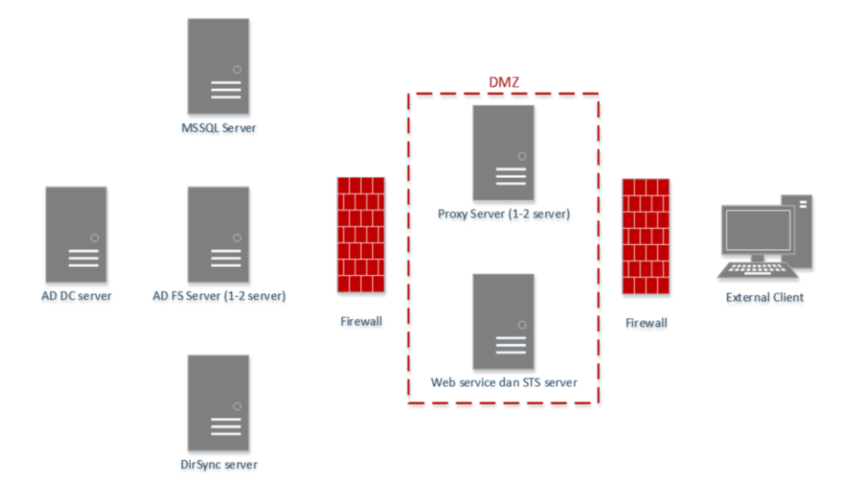
\includegraphics[width=12cm]{contents/chapter-2/gambar-buatan-sendiri.png}
	\caption{Contoh gambar}
	\label{Fig:gambar-buatan-sendiri}
\end{figure}

\textit{Game design document} adalah sebuah bagian penting dalam pembuatan game baik itu elemen-elemen penyusunnya maupun proses pengembangannya. Game design yang telah dibuat, dijabarkan satu persatu mengenai tahapan dalam pembuatan game dan hasilnya disatukan dalam bentuk dokumentasi \textit{game design document} yang digunakan oleh \textit{developer} sebagai buku petunjuk bagaimana membuat \textit{game} \cite{lukito2016}.

Dalam buku \textit{Game Design Essentials} disebutkan \textit{game design document} merupakan metode yang menghubungkan elemen-elemen penyusun \textit{game}, baik itu \textit{art, sound, program, 
gameplay} sehingga semuanya terdokumentasi menjadi satu dan menjadi acuan bagi para \textit{developer} dalam membuat \textit{game} \cite{wibirama2013dual}. 

\cleardoublepage \phantomsection
\chapter{Metode Penelitian}

Bab ini menjelaskan metode atau cara yang digunakan dalam penelitian ini untuk 
mencapai maksud dan tujuan seperti yang tertulis dalam sub-bab 1.3 [jika diinginkan, kalian dapat menuliskan Kembali tujuan penelitian yang ingin dicapai di sini].

\section{Metode yang Digunakan}

Bagian ini membahas metode atau cara yang akan digunakan dalam penelitian, tahapan 
penerapan metode, dan desain penelitian (misalnya apakah penelitian akan menggunakan 
eksperimen di Laboratorium atau di lapangan, misalkan saja penelitian biomedis atau 
penelitian alat ukur hama yang dapat dilakukan di laboratorium ataupun di lapangan, atau menggunakan metode survei (misalnya untuk teknologi Informasi), studi kasus, atau analisisdengan perangkat lunak (ETAP, LT Spice, dst), atau \textit{prototyping} (pembuatan perangkat keras).

\section{Alat dan Bahan Tugas akhir}

\subsection*{Alat Tugas akhir}

Alat-alat yang digunakan pada tugas akhir ini berupa perangkat keras maupun perangkat lunak sebagai sarana pendukung antara lain. Kemukakan secara detail sesuai dengan kebutuhan tugas akhir dan juga tambahkan spesifikasi minumum sehingga peneliti lain yang hendak melakukan hal yang sama bisa melakukannya :

\begin{enumerate}
\item \textit{Notebook} dengan spesifikasi minumum sistem operasi Windows 8, \textit{processor} Intel Core i3 2330M CPU @ 2,2 GHz, memori 4GB DDR3, grafis NVIDIA GeForce GT 610 (4GB), hardisk 500GB. Pada tugas akhir ini digunakan Windows 10, Intel Core i7 4570M CPU, Memori 4GB DDR 3, grafis Intel HD4300. 
\item \textit{Smartphone} dengan spesifikasi tipe minimum, OS Android OS v4.1.2 (Jelly Bean),CPU Dual-core 800 MHz, GPU Mali-400, Internal 4 GB, 768 MB RAM. Pada tugas akhir ini digunakan ....
\item \textit{Game creation platform} versi 3.3.2 untuk Stencyl dan Construct2.
\item CORELDRAW X7, Tiled dan GIMP 2
\end{enumerate}

\subsection*{Bahan Tugas akhir}

Bahan tugas akhir adalah segala sesuatu yang bersifat fisik atau digital yang digunakan untuk kebutuhan tugas akhir. Bahan tugas akhir dapat berupa:

\begin{enumerate}
\item Bahan habis pakai. Bahan yang digunakan untuk tugas akhir. Sebagai contoh 
mungkin dibutuhkan kertas transparansi, baterai, atau yang lain 
\item Bahan yang berupa data atau informasi yang menjadi dataset tugas akhir. Dataset tugas akhir dapat berupa:
\end{enumerate}
	\begin{itemize}
	\item Dataset pihak lain yang diperoleh dengan izin atau dalam lisensi yang diizinkan untuk digunakan secara langsung 
	\item Dataset pihak pertama yang disusun sendiri melalui quisioner, observasi, atau interview 
	\item Dokumen panduan yang mengacu pada standar, hasil tugas akhir, atau artikel yang disitasi dan digunakan.
	\end{itemize}

\section{Alur Tugas Akhir}

Menguraikan prosedur yang akan digunakan dan jadwal atau alur penyelesaian setiap 
tahap. Alur penelian ini dapat disajikan dalam bentuk diagram. Diagram dapat disusun dengan aturan yang baik semisal menggunakan Flowchart. Aturan dan tutorial pembuatan flowchart dapat dilihat di \textcolor{blue}{http://ugm.id/flowcharttutorial}. Setelah menggambarkannya, penulis wajib menjelaskan langkah-langkah setiap alur tugas akhir dalam sub bab tersendiri sesuai dengan kebutuhan.

\section{Metode Analisis Data}

Bagian ini membahas bagaimana data [akan] dianalisis, apakah dengan membandingkan 
keluaran beberapa alat ukur, membandingkan dengan standar atau bagaimana.

\section{Etika, Masalah dan Keterbatasan Penelitian (khususnya untuk Teknik Biomedis)}

Bagian ini membahas pertimbangan etis penelitian dan [potensi] masalah serta
keterbatasannya. Jika menyangkut penelitian dengan makhluk hidup, maka dibutuhkan adanya \textit{ethical clearance}, di bagian ini hal itu akan dibahas. Demikian juga tentang keterbatasan ataupun masalah yang akan timbul.

\cleardoublepage \phantomsection
\chapter{Hasil dan Pembahasan}

\section{Pembahasan Hasil 1 (Ubah Judul Sesuai dengan Hal yang Hendak dibahas)}

Poin pertama adalah membahas tujuan penelitian pertama. 
Dapat ditambahkan beberapa sub bab jika diperlukan.

\section{Pembahasan Hasil 2 (Ubah Judul Sesuai dengan Hal yang Hendak dibahas)}

Poin kedua adalah membahas tujuan penelitian kedua. Dapat ditambahkan beberapa 
sub bab jika diperlukan. Dapat juga diteruskan ke Sub Bab Pembahasan hasil 3 dan 
seterusnya, jika ada tiga atau lebih tujuan penelitian.

\section{Perbandingan Hasil Penelitian dengan Hasil Terdahulu}

Pembahasan penutup dapat menjelaskan mengenai kelebihan hasil pengembangan / 
penelitian dan kekurangan dibandingkan dengan skripsi atau penelitian terdahulu atau
perbandingan terhadap produk lain yang ada di pasaran. Penulis dapat menggunakan tabel untuk membandingkan secara gamblang dan menjelaskannya.
\cleardoublepage \phantomsection
\chapter{Kesimpulan dan Saran}

\section{Kesimpulan}

Kesimpulan dapat diawali dengan apa yang dilakukan dengan tugas akhir ini lalu 
dilanjutkan dengan poin-poin yang menjawab tujuan penelitian, apakah tujuan sudah tercapai atau belum, tentunya berdasarkan data ataupun hasil dari Bab pembahasan sebelumnya. Dalam beberapa hal, kesimpulan dapat juga berisi tentang temuan/\textit{findings} yang Anda dapatkan setelah melakukan pengamatan dan atau analisis terhadap hasil penelitian. 

\section{Saran}

Saran berisi hal-hal yang bisa dilanjutkan dari penelitian atau skripsi ini, yang belum dilakukan karena batasan permasalahan. Saran bukan berisi saran kepada sistem atau pengguna, tetapi saran diberikan kepada aspek penelitian yang dapat dikembangkan dan ditambahkan di penelitian atau skripsi selanjutnya.

\cleardoublepage \phantomsection
\chapter{Kesimpulan dan Saran}

\section{Kesimpulan}

Kesimpulan dapat diawali dengan apa yang dilakukan dengan tugas akhir ini lalu 
dilanjutkan dengan poin-poin yang menjawab tujuan penelitian, apakah tujuan sudah tercapai atau belum, tentunya berdasarkan data ataupun hasil dari Bab pembahasan sebelumnya. Dalam beberapa hal, kesimpulan dapat juga berisi tentang temuan/\textit{findings} yang Anda dapatkan setelah melakukan pengamatan dan atau analisis terhadap hasil penelitian. 

\section{Saran}

Saran berisi hal-hal yang bisa dilanjutkan dari penelitian atau skripsi ini, yang belum dilakukan karena batasan permasalahan. Saran bukan berisi saran kepada sistem atau pengguna, tetapi saran diberikan kepada aspek penelitian yang dapat dikembangkan dan ditambahkan di penelitian atau skripsi selanjutnya.


%======================================

%======================================
%  References
%======================================
\cleardoublepage \phantomsection
\thereferences
% You can change 
%    the filename and location of the files inputted
\bibliography{references}

%Hapus bagian di bawah setelah tidak diperlukan
\begin{center}
	\textcolor{red}{
	Catatan: Daftar pustaka adalah apa yang dirujuk atau disitasi, bukan apa yang telah dibaca, jika tidak ada dalam sitasi maka tidak perlu dituliskan dalam daftar pustaka.}
\end{center}

%======================================

%======================================
%  Appendix
%======================================
% You can change 
%    the filename and location of the files inputted
%    use \chapterappendix for the first page of the appendix
%    use \chapterappendixadd for the next page

\appendix

\cleardoublepage \phantomsection
\chapterappendix{contents/appendix/appendix-isi-lampiran}
\chapterappendixadd{contents/appendix/appendix-latex}
\chapterappendixadd{contents/appendix/appendix-penulisan-referensi}
\chapterappendixadd{contents/appendix/appendix-code}




%======================================

\end{document}